\documentclass[dvipdfmx,uplatex]{jsarticle}

%% Packages
\usepackage{graphicx,color,hyperref}
\usepackage{algorithm}
\usepackage{algorithmic}
\usepackage{url}
\usepackage{lscape}
\usepackage{mathtools}
\usepackage{here}
\usepackage{amsmath,amssymb,amsfonts}
\usepackage{amsthm}
\usepackage{tikz}
\usepackage{tcolorbox}
\usepackage{pxjahyper}

%% Theorem Styles
\newtheorem{theorem}{定理}
\newtheorem{proposition}{命題}
\newtheorem{cor}{系}
\newtheorem{definition}{定義}
\newtheorem{problem}{問題}
\theoremstyle{remark}
\newtheorem{remark}{注意}
\newtheorem{requirement}{条件}

%% Environment (Colorful Box)
\newenvironment{simplebox}{
    \begin{tcolorbox}[
        fonttitle=\bfseries,
    ]
}{
    \end{tcolorbox}
}

\newenvironment{method}[1]{
    \begin{tcolorbox}[
        colframe=green!50!black,
        colback=green!50!black!10!white,
        colbacktitle=green!50!black!40!white,
        coltitle=black,
        fonttitle=\bfseries,
        title={#1}
    ]
}{
    \end{tcolorbox}
}

\newenvironment{experiment}[1]{
    \begin{tcolorbox}[
        colframe=violet,
        colback=violet!10!white,
        colbacktitle=violet!40!white,
        coltitle=black,
        fonttitle=\bfseries,
        title={#1}
    ]
}{
    \end{tcolorbox}
}

\newenvironment{kansou}{
    \begin{tcolorbox}[
        colframe=brown,
        colback=brown!10!white,
        colbacktitle=brown!40!white,
        coltitle=black,fonttitle=\bfseries
    ]
}{
    \end{tcolorbox}
}

%% Title
\title{Dremel: interactive analysis of web-scale datasets}
\author{\empty}
\date{\empty}

%% Document body
\begin{document}
\maketitle

\begin{itemize}
    \item Link: \url{https://dl.acm.org/doi/10.14778/1920841.1920886}
    \item Conference: VLDB2010
    \item Citation: \cite{dremel_2010}
    \item Google User Content: \url{https://static.googleusercontent.com/media/research.google.com/en//pubs/archive/36632.pdf}
\end{itemize}

\section{概要}
\begin{simplebox}
\begin{itemize}
    \item dremelはスケーラブルでインタラクティブなクエリシステムである。dremelはカラム型データレイアウトとマルチレベル実行ツリーを組み合わせることで、数兆行規模のテーブルに対する集約クエリを数秒で実行できる。
    \item この論文ではdremelのアーキテクチャ、実装について説明し、実際に数千ノード規模のインスタンスで行った実験について議論する。
\end{itemize}
\end{simplebox}

\section{背景}
\begin{simplebox}
\begin{itemize}
    \item ストレージが低価格化したことで、多くのデータを保持できるようになり、それによって大量のデータを高速に分析することは重要になってきた。
    \item またWebで扱われるデータは非リレーショナルででネストされたデータモデルに基づくことが多い。
    \item 本論文ではDremelというシステムを紹介する。これは共有クラスタ上で大規模なデータセットの分析を可能にするものである。
\end{itemize}
\end{simplebox}

\section{手法}
\begin{method}{データモデル}
\begin{itemize}
    \item データは次のようなネストされたデータであらわされる。この形はProtocol Buffersの由来で生まれたものである。
    \item $\tau = \mathrm{dom} | \langle A_1: \tau[*|?], \dots, A_n: \tau[*|?] \rangle$で、$\tau$であらわされる。($\mathrm{dom}$は原始型でこれは整数、浮動小数点、文字列などが含まれる、$A_i$はフィールドの名前、$*$は繰り返し、$?$はオプショナルを表す)
\end{itemize}
\end{method}

\begin{figure}
    \centering
    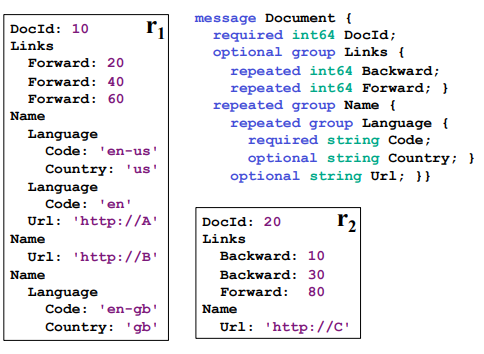
\includegraphics[width=0.5\textwidth]{img/dremel/schema.png}
    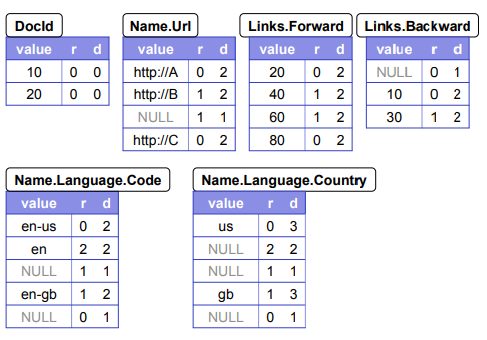
\includegraphics[width=0.5\textwidth]{img/dremel/repeat.png}
    \caption{ネスト型スキーマとその表現の例}
    \label{fig:dremel_schema}
\end{figure}

\begin{method}{ネスト型カラムストレージ}
\begin{itemize}
    \item ネストされたデータをカラム形式で保存するには、各フィールドに対して列を作成する。繰り返しフィールドもあるため、どのようにそれらを表現するかという問題が生じる。これを二つのレベルを使って表現する。
    \item Repetition level
    \begin{itemize}
        \item Repetition levelは、どのレベルの繰り返しフィールドが繰り返されたことでその値が現れたかを示す。
        \item e.g. 図\ref{fig:dremel_schema}の例では、Name.Language.Codeでは、"en-us"では繰り返しなしのため0, "en"ではLanguageが繰り返されたため(Languageの深さはName.Languageで2なので)2、"en-gb"では直近でNameが繰り返されたので1となる。
    \end{itemize}
    \item Definition level
    \begin{itemize}
        \item Definition levelは、そのフィールドを定義するパスのなかで未定義になり得るフィールドの内、実際にレコード内で存在するものの数を表す
        \item e.g. 図\ref{fig:dremel_schema}の例では、r1にはBackwardリンクが存在しないが、Linksフィールド自体は定義されているため、Link.BackwardにはDefinition levelが1のNULLを追加する。
    \end{itemize}
    \item 上のレベルは必要なもののみ保存することで、ストレージのオーバーヘッドを抑えることができる。
    \item ネストされたレコードからカラムへの分割は再帰的に行うことで可能になる。
    \item カラムで表現されたレコードから、ラベルの部分集合を与えられて、そのレコードのラベルに対応する値を抽出する、これはFSM(有限状態機械)で行う。
    \begin{itemize}
        \item FSMの状態は、現在のレコードのどの部分にいるかを表し、Repetition levelをつかって状態遷移を行う。
        \item レコード全体を取得する場合と必要なフィールドの部分集合のみ取得する場合でFSMを変えることで、必要なフィールドのみを効率的に取得できる。
    \end{itemize}
\end{itemize}
\end{method}

% \begin{method}{クエリ言語}
% \begin{itemize}
%     \item 
% \end{itemize}
% \end{method}

\begin{figure}
    \centering
    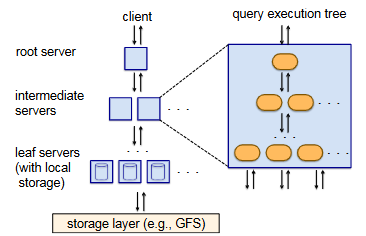
\includegraphics[width=0.5\textwidth]{img/dremel/execution.png}
    \caption{クエリ実行時のアーキテクチャ}
    \label{fig:query-execution}
\end{figure}

\begin{method}{クエリ実行}
\begin{itemize}
    \item DremelにおけるクエリはSQLに似た言語で書かれる。
    \item Tree Architecture
    \begin{itemize}
        \item クエリ実行はツリー型のアーキテクチャで行われる(図\ref{fig:query-execution})、テーブルを構成するタブレットを決定し、クエリを書き換え、クエリを実行し、結果を集約することで実行する。 
    \end{itemize}
    \item Query Dispatcher
    \begin{itemize}
        \item Dremelはマルチユーザのシステムで、通常は複数のクエリが同時に発行される。クエリディスパッチャは優先度に基づいたスケジューリング、負荷分散などを行う。
        \item リーフサーバはカラム表現されているネストデータをストライプ単位で(テーブルをいくつかに行方向に分割した単位で)読みこむ、そのあとにその結果を集約することで最終的な結果を得る。またその実行計画はできるだけレコードの組み立てを回避するように設計されている。
    \end{itemize}
\end{itemize}
\end{method}

\section{実験結果}

\begin{figure}
    \centering
    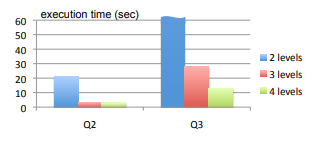
\includegraphics[width=0.5\textwidth]{img/dremel/serving-tree.png}
    \caption{サービングツリーの深さと実行時間の関係}
    \label{fig:serving-tree}
\end{figure}

\begin{figure}
    \centering
    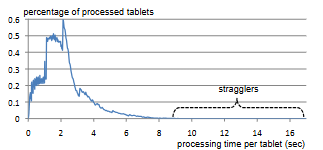
\includegraphics[width=0.5\textwidth]{img/dremel/stragglers.png}
    \caption{Stragglerの存在}
    \label{fig:straggler}
\end{figure}

\begin{experiment}{実験結果}
\begin{itemize}
    \item いくつかのGoogleで使用されているデータセットに対してDremelの性能を評価し、カラム型ストレージでの有効性を検証する。
    \item フィールドのエンコーディングの比較
    \begin{itemize}
        \item 本論文のカラム型ストレージと、レコード指向ストレージのデータのRead/Writeの性能を比較する、フィールドの部分集合を対象にデータの読み取り、解凍、レコードの組み立てを行う時間を比較する。
        \item 少数のカラムを読む場合はカラム型表現は1桁の性能向上をもたらす。
    \end{itemize}
    \item MapReduceとDremelの比較
    \begin{itemize}
        \item カラム型フォーマット、レコード指向フォーマットの二つでMapReduce, Dremelの性能を比較する。この実験では一つのカラムだけ読むクエリを実行する。
        \item まずカラム型フォーマットとレコード指向フォーマットでは読み出しレコード量が大きく異なる。
        \item さらにDremelのツリーアーキテクチャとMapReduceのアーキテクチャを比較すると、Dremelの方が高速だった。
    \end{itemize}
    \item サービングツリーのトポロジー
    \begin{itemize}
        \item サービングツリーの深さを変化させたときのクエリ実行時間を比較する。次の二つのクエリで比較する。Q2: SELECT country, SUM(item.amount) FROM T2 GROUP BY countryとQ3: SELECT domain, SUM(item.amount) FROM T2 WHERE domain CONTAINS '.net' GROUP BY domainである。
        \item 実験結果は図\ref{fig:serving-tree}のようになった。いずれの場合でもレベルが2から3に増えると精度が大幅に向上する、これはレベル2ではルートサーバが多数のノードからの結果を集約しなければならないからである。
        \item Q2ではレベルが2から3に増えてもそれほど改善しないが、Q3では大幅に改善する、これはQ3のほうが集約するグループがおおく並列化の恩恵を受けやすいためである。
    \end{itemize}
    \item レコード内集約
    \begin{itemize}
        \item 次のようなクエリを実行し、レコード内集約がどのように効くかを評価する。Q4: SELECT COUNT(c1 > c2) FROM (SELECT SUM(a.b.c.d) WITHIN RECORD AS c1, SUM(a.b.p.q.r) WITHIN RECORD AS c2 FROM T3)
        \item この実験で用いたデータセットではこのクエリで70TB中13GBのみを読みこみ、15秒でクエリを実行した。ネストに対応しないようなカラムフォーマットである場合このクエリは非常に高コストになる。
    \end{itemize}
    \item Stragglers
    \begin{itemize}
        \item Stragglers(極端に遅いノード)が存在することを実験で示す。クエリQ5: SELECT COUNT(DISINTCT a) FROM T5を実行して、各ノードの実行時間を測定すると図\ref{fig:straggler}のようになり、多くのノードは短い時間で処理されるが、ごく一部は極端に遅いことがわかる。
    \end{itemize}
\end{itemize}
\end{experiment}

\section{感想}
\begin{kansou}
\begin{itemize}
  \item BigQueryのもとになった技術であるDremelの論文で、面白かった。
  \item ネストされているレコードをカラム形式で保存する手法でカラムからネストされた型へのデコードとエンコードを有限状態機械で行うというのが面白かった。取得したいフィールドに応じてFSMを変化させて、効率的に取得するようになっているのも面白い。たぶんこのネストされたデータをカラム形式で保存する手法が肝な気がする。
  \item MapReduceとDremelのツリー構造のアーキテクチャは異なって、ユースケースごとに最適な形が異なるのだろうと感じた。MapReduceはもっと大規模なバッチ処理向きで、Dremelは中規模くらいのデータでの処理向きな感じがした。
\end{itemize}
\end{kansou}

% \begin{figure}
%     \centering
%     
\includegraphics[width=0.5\textwidth]{img/image.png}
%     \caption{キャプション}
%     \label{fig:template}
% \end{figure}

\bibliographystyle{jplain}
\bibliography{template.bib}

\end{document}